\documentclass{article}

\usepackage{graphicx}
\usepackage{amssymb}
\usepackage{lastpage}
\usepackage{epstopdf}
\usepackage{fancyhdr}
\DeclareGraphicsRule{.tif}{png}{.png}{`convert #1 `dirname #1`/`basename #1 .tif`.png}

\newcommand{\cAuthor}{Raphael Sofaer}
\newcommand{\cTitle}{Trendlines and numerical issues in Google Spreadsheet}
\pagestyle{fancy}
\lhead{\cAuthor}                                                 %
\rhead{\cTitle}  %
\lfoot{\lastxmark}                                                      %
\cfoot{}                                                                %
\rfoot{Page\ \thepage\ of\ \pageref{LastPage}}                          %
\renewcommand\headrulewidth{0.4pt}                                      %
\renewcommand\footrulewidth{0.4pt}        

\title{\cTitle}
\author{\cAuthor}
\begin{document}
\maketitle

\section*{Abstract}
Google Spreadsheet is an online spreadsheet program in the style of Microsoft Excel.
It provides much of Excel's data management and charting functionality, though not all,
and also allows spreadsheets to be shared and edited cooperatively.
Perhaps the most powerful feature of Google Spreadsheets is the API,
which allows the owner of a spreadsheet to programatically modify and read it.
Using that API, Google Spreadsheet can provide a turnkey and user friendly window into
arbitrary data as it is gathered.  The number of Google apps users is growing,
with at least 40 million users\footnote{Google Apps for Enterprise: http://www.google.com/enterprise/apps/business/}
that have apps accounts, and some of those users
will depend on Spreadsheet's accuracy for their business.  This paper will examine
Google Spreadsheet's accuracy at computing linear best fit lines with ill-conditioned data,
comparing it with GNU Octave and Antony Kaplan's work on Excel
\footnote{Kaplan 2010 http://cs.nyu.edu/courses/spring12/CSCI-UA.0421-001/kaplanproject.pdf}
as well as some related quirks of Google Spreadsheet.
\newpage
\section*{Floating Point Numbers in Google Spreadsheet}
It can be difficult to tell what sort of floating point math a spreadsheet program uses.
Microsoft Excel, for instance, uses cosmetic rounding to make binary floating point numbers
appear to be decimal floating point numbers
\footnote{How Futile are Mindless\dots: http://www.cs.berkeley.edu/~wkahan/Mindless.pdf}.
Google, on the other hand, made no attempt to confirm or deny the floating-point truth.
To the best of my knowledge, exhibited below, Google uses software implemented decimal floating point.\\

If we look at the edge of Google Spreadsheet's precision in binary, we see that
$1 + 2^{-46} = 1 + 2^{-47} \ne 1$.  This suggests that Google's floating point is not in the form $m*2^{x}$.\\
\begin{table}[h!]
  \centering
    \begin{tabular}{|l|l|l|l|l|}
  \multicolumn{5}{c}{The edge of Google Spreadsheet's precision with binary floating point:}\\
  \hline
        i  & $2^{-i}$          &  $1 + 2^{-i}$    & $1 = 1 + 2^{-i}$ & $1 + 2^{-i} = 1 + 2^{-(i+1)}$ \\
        \hline
        44 & 0.000000000000057 & 1.00000000000006 & FALSE & FALSE \\ 
        45 & 0.000000000000028 & 1.00000000000003 & FALSE & FALSE \\ 
        46 & 0.000000000000014 & 1.00000000000001 & FALSE & TRUE  \\ 
        47 & 0.000000000000007 & 1.00000000000001 & FALSE & FALSE \\ 
        48 & 0.000000000000004 & 1                & TRUE  & TRUE  \\ 
        49 & 0.000000000000002 & 1                & TRUE  & TRUE  \\ 
        50 & 0.000000000000001 & 1                & TRUE  & TRUE  \\ 
        51 & 0                 & 1                & TRUE  & TRUE  \\
        \hline
    \end{tabular}
\end{table}

In decimal we see no such irregularities:
\begin{table}[h!]
  \centering
    \begin{tabular}{|l|l|l|l|l|}
        \multicolumn{5}{c}{The edge of Google Spreadsheet's precision with decimal floating point:}\\
        \hline
        i  & $10^{-i}$          &  $1 + 10^{-i}$    & $1 = 1 + 10^{-i}$ & $1 + 10^{-i} = 1 + 10^{-(i+1)}$ \\
        \hline
        12 & 0.000000000001    & 1.000000000001   & FALSE & FALSE \\
        13 & 0.0000000000001   & 1.0000000000001  & FALSE & FALSE \\ 
        14 & 0.00000000000001  & 1.00000000000001 & FALSE & FALSE \\ 
        15 & 0.000000000000001 & 1                & TRUE  & TRUE  \\
        \hline
    \end{tabular}
\end{table}

\newpage
This gives us a few identities:\\
$$1 + 2^{-47} \ne 1$$
$$1 + 2^{-48} = 1$$
$$1 + 2^{-46} = 1 + 2^{-47} = 1 + 10^{-14}$$
$$1 = 1 + 10^{-15}$$

Where Excel used hardware binary floating point and hushed it up, Google seems to have implemented 
true decimal floating point.

\section*{The TREND function}
Google Spreadsheet's basic linear best fit function is TREND(data\_X,data\_Y,x).
Given two vectors of data, it calculates the value of the linear best fit at x.
However, as the data it is given becomes ill conditioned, the accuracy of TREND
desintigrates.  Here we examine data series' of the form ${(1 + i/10^{-j}, i + 1)}$,
where $i$ ranges from 0 to 12.\\
\begin{table}[h!]
  \centering
    \begin{tabular}{|l|l|l|}
        \multicolumn{3}{c}{Data series for j=6}\\
        X Values   & Y values & Trendline        \\
        1          & 1        & 1                \\ 
        1.00000001 & 2        & 1.93142622709274 \\ 
        1.00000002 & 3        & 2.86285246908665 \\ 
        1.00000003 & 4        & 3.79427869617939 \\ 
        1.00000004 & 5        & 4.72570492327213 \\ 
        1.00000005 & 6        & 5.65713113546372 \\ 
        1.00000006 & 7        & 6.58855739235878 \\ 
        1.00000007 & 8        & 7.51998360455036 \\ 
        1.00000008 & 9        & 8.4514098316431  \\ 
        1.00000009 & 10       & 9.38283605873585 \\ 
        1.0000001  & 11       & 10.3142623007298 \\ 
        1.00000011 & 12       & 11.2456885278225 \\ 
        1.00000012 & 13       & 12.1771147549152 \\
    \end{tabular}
\end{table}

\newpage
When $j=0$, there is no numerical error ($R^2=1$).
However, by the time $j=5$, we begin to see error creep into the numbers ($R^2 = 0.999999999999965$).
By the time $j=7$, only one correct decimal place remains,
creating barely visible error ($R^2=0.99999438640566$).\\
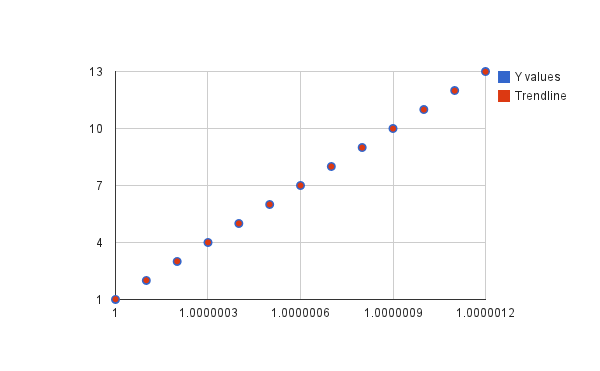
\includegraphics[width=4in]{TRENDj7.png}\\
When $j=8$, the trendline has ventured out alone, with an $R^2$ value of $0.983604355317896$.\\
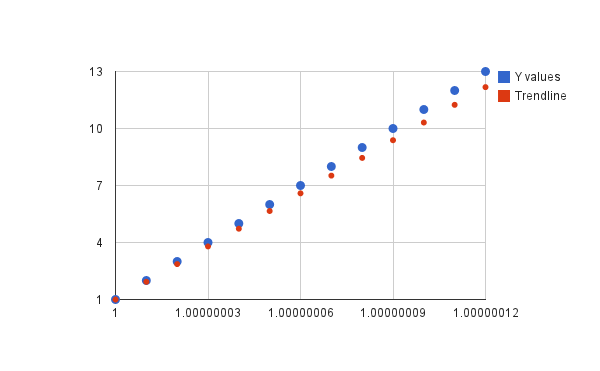
\includegraphics[width=4in]{TRENDj8.png}\\
\newpage
At $j=9$, there is only madness.  Rather than a slope of $10^{j}$,
the trendline has a small negative slope, and $R^2 =-0.078210891033562$.\\
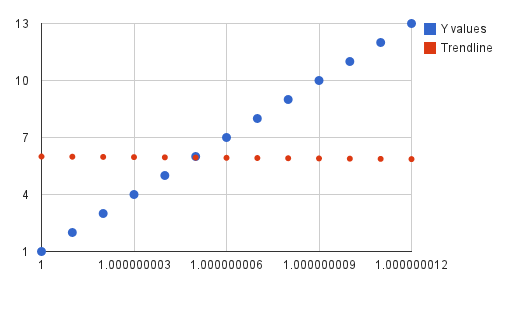
\includegraphics[width=4in]{TRENDj9.png}\\
At $j=10$, the spreadsheet crashes, and the page reloads,
with the change forgotten.  This is a consistent result.\\

By contrast, GNU Octave performs perfectly
\footnote{Code used: ex = j; x = 1+0*10\^-ex:10\^-ex:1+12*10\^-ex; y = 1:13;[b,s,r] = ols(y,x);plot(x,y,x,x*b);axis([1 x(size(x)(2)) 0 14]);}
up to $j=14$, the edge of its numerical precision.\\
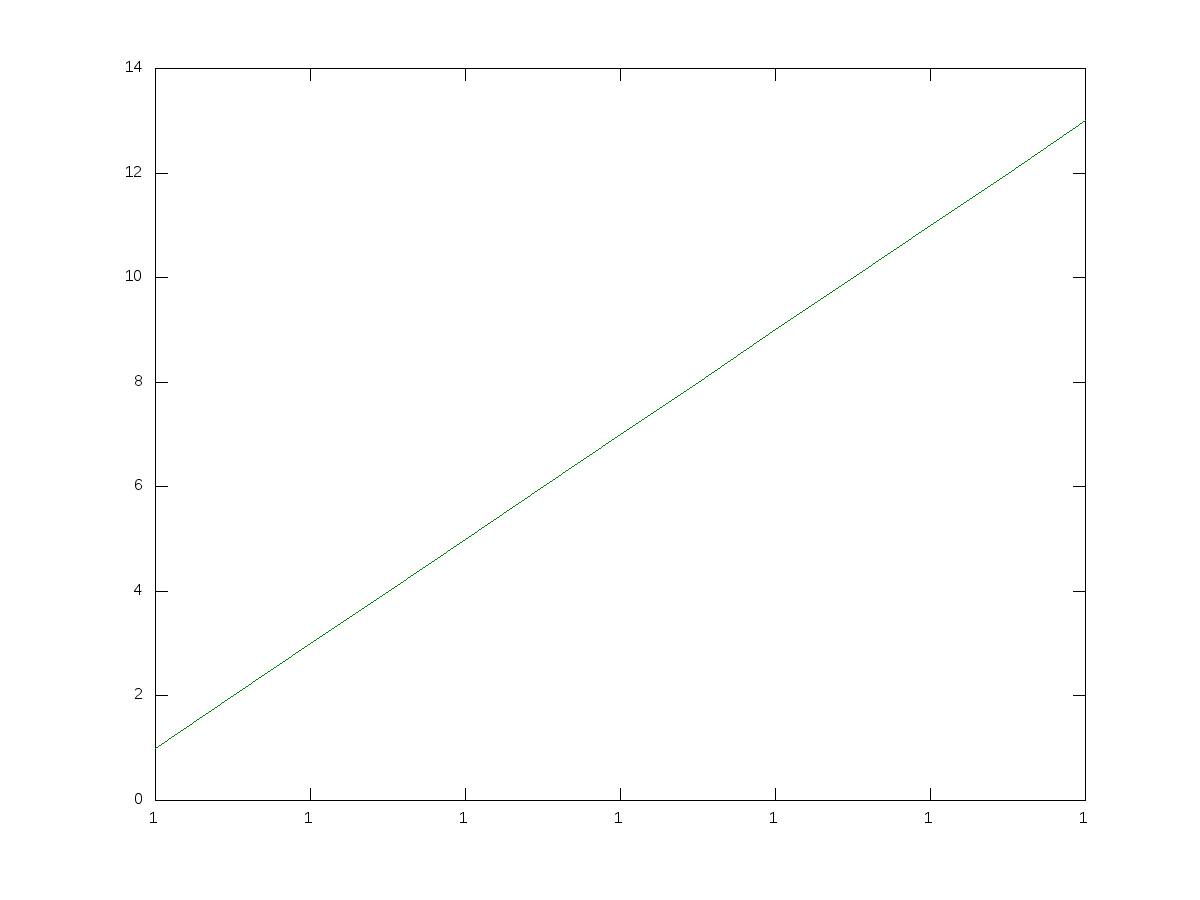
\includegraphics[width=4in]{TRENDocj14.png}\\
\newpage
Only when $j=15$ does Octave begin to reveal the underlying discrete nature of floating point.\\
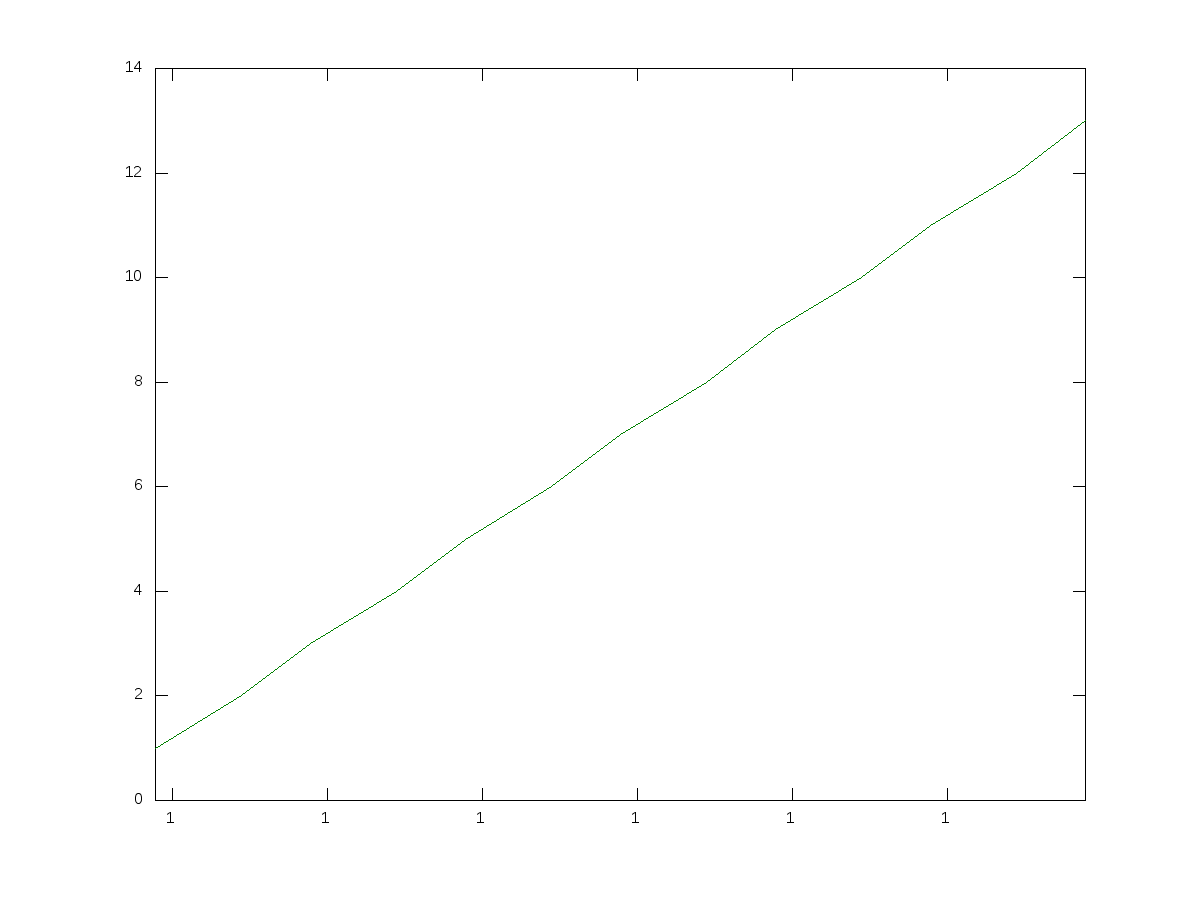
\includegraphics[width=4in]{TRENDocj15.png}\\
At $j=16$, Octave finally has an error and displays nothing, but there is no crash, and 
the failure to produce an answer makes sense, as $10^{-16}$, the spacing of the x coordinates,
is $\approx \epsilon/2$, where $\epsilon$ is provided in Octave as eps.

For better comparison with Kaplan's work on Excel, we also examined data series'
of the form ${(1 + (i + 40)/2^{-j}, i)}$, where $1\le i \le 8$.
Kaplan found that Excel's Trendline function only performed well with $j \le 25$,
with bad error up to $j \le 27$, and various degrees of failure past that.


\section*{Conclusion}




\end{document}
